  %%%%%%%%%%%%%%%%%%%%%%%%%%%%%%%%%%%%%%% -*- coding: utf-8; mode: latex -*- %%
  %
%%%%%                         CHAPTER
 %%%
  %

% $Id: 1020-lorem-ipsum.tex,v 1.2 2009/06/19 15:51:46 david Exp $
% $Log: 1020-lorem-ipsum.tex,v $
% Revision 1.2  2009/06/19 15:51:46  david
% *** empty log message ***
%
% Revision 1.1  2007/11/23 09:52:39  david
% *** empty log message ***
%
%

  %%%%%%%%%%%%%%%%%%%%%%%%%%%%%%%%%%%%%%%%%%%%%%%%%%%%%%%%%%%%%%%%%%%%%%%%%%%%%
  %
%%%%%                           HEAD MATTER
 %%%
  %
\chapter{Solution}
\label{ch:solution}

\section{Operations to Support}

\begin{enumerate}
\item All file system operations are allowed on the snapshotted file/directories including:\\
\hspace{5em} Rename is allowed both within and across snapshottable directory boundaries.

\item Any modification to the current files or directories are not reflected in the snapshots. The
snapshot is read-only.\\
\hspace{5 em} The modification include length change, renaming of the file name, permission changes or any other attribute changes such as replication factor etc.

\item The snapshot files and directories can be only be read, not modified in any way (except that the
entire snapshot can be deleted). This means the replication factor, permission or any other
attributes of file or directory cannot be changed. The snapshots are truly read-only.

\item Nested snapshots are allowed.

\item Access time is not tracked for snapshots.

\item Snapshots should be created very fast.

\item Block data is not copied for snapshots

\end{enumerate}


\section{Read-Only Nested Snapshots}
%\addcontentsline{lof}{chapter}{\thechapter\quad Lorem Ipsum}
%\addcontentsline{lot}{chapter}{\thechapter\quad Lorem Ipsum}


  %%%%%%%%%%%%%%%%%%%%%%%%%%%%%%%%%%%%%%%%%%%%%%%%%%%%%%%%%%%%%%%%%%%%%%%%%%%%%
  %
%%%%%                        FIRST SECTION
 %%%
  %
\subsection{Snapshottable Directories}

 These are directories that are configured
by the system administrator to allow snapshots. A snapshot can be created only at these snapshot roots
instead of at arbitrary directories.
Directories that are marked snapshottable cannot be deleted until all the snapshots under that directory
are deleted. Similarly, another directory cannot be renamed to an existing a snapshottable directory
that has snapshots (since rename involves deletion of the rename target). The above restrictions
simplify the design by not having to deal with how to mange a snapshot when the snapshottable
directory is deleted and no longer exists or worst still a new directory with the same name is created in
its place.

\subsection{Modifications to the Schema}
\label{RONSS:schema}

Following columns need to be added to the Inodes table described in the schema \ref{fig:HDFS_table_schema} of HOP File System.
\begin{enumerate}
\item isDeleted \\\\
\begin{tabular}{|c|p{15cm}|}
\hline
Value&Summary\\
\hline
0&Indicates that this Inode is not deleted.\\
\hline
1&Indicates that this Inode deleted after snapshot was taken[on its ancestors].\\ 
\hline
\end{tabular} \\
\item isSnapshottableDirectory\\\\
\begin{tabular}{|c|p{15cm}|}
\hline
Value&Summary\\
\hline
0&Indicates that snapshots can't be taken on this directory.\\
\hline
1&Indicates that snapshots can be taken on this directory.\\ 
\hline
\end{tabular} \\
\end{enumerate}
Following tables need to be added to the schema \ref{fig:HDFS_table_schema}.
\begin{enumerate}
\item \textbf{SNAPS}\\\\
\begin{tabular}{|c|c|c|c|}
\hline
Inode\_ Id&
User&
SnapShot\_ Id&
Time\\
\hline
\end{tabular}\\\\
Stores the Indode Id and corresponding snapshots taken on that directory. Time can be a physical clock or logical clock(Global) whose value always increase.

\item \textbf{C-List}\\\\
\begin{tabular}{|c|c|c|}
\hline
Inode\_ Id&
Time&
Created\_ Inode\_ Id\\
\hline
\end{tabular}\\\\
Stores the id's of children(files or directories) of directory on which snapshot was taken.



\item \textbf{D-List}\\\\
\begin{tabular}{|c|c|c|}
\hline
Inode\_ Id&
Time&
Deleted\_ Inode\_ Id\\
\hline
\end{tabular}\\\\
Stores the  files or directories  deleted in a directory on which snapshot was taken. But the rows are not deleted from Inode table, it is an indication to say that these rows were deleted after taking snapshots.

\item \textbf{M-List}\\\\
\begin{tabular}{|c|c|c|c|}
\hline
Inode\_ Id&
Time&
Modified\_ Inode\_ Id&
Original Row\\
\hline
\end{tabular}\\\\
After taking a Snapshot if the columns of a particular row are modified then before modifying the row , we copy the original row and store it in this table. When we want to get back to the snapshot, just replace the existing inode row with this original row.

\item \textbf{MV-List}\\\\
\begin{tabular}{|c|c|c|c|}
\hline
Inode\_ Id&
Time&
Moved\_ Inode\_ Id&
Original Row\\
\hline
\end{tabular}\\\\
When an inode[either file or directory] is moved, its parentId changes to moved-into directory. In order to get the moved directory when ls command issued at the snapshot after which this inode was moved, we put that row here. 

\item \textbf{MV-IN-List}\\\\
\begin{tabular}{|c|c|c|c|}
\hline
Inode\_ Id&
Time&
Moved\_ In\_ Inode\_ Id\\
\hline
\end{tabular}\\\\
When a directory or file is moved into this directory(with inode\_ id) from other directory.

\item \textbf{Block-Info-C-List}\\\\
\begin{tabular}{|c|c|c|}
\hline
Inode\_ Id&
Block\_ Id&
Time\\
\hline
\end{tabular}\\\\
Stores the blocks that are created in a file after the snapshot was taken on the directory in which this file exist.

\item \textbf{Block-Info-M-List}\\\\
\begin{tabular}{|c|c|c|c|}
\hline
Inode\_ Id&
Block\_ Id&
Time&
Original\_ Row\\
\hline
\end{tabular}\\\\
Stores the blocks that are modified in a file after the snapshot was taken on the directory in which this file exist.This is typically for last blocks which are not complete at the time of snapshot.

\end{enumerate}

\subsection{Rules for Operations}
\begin{enumerate}

\item  When we create a new file or directory put an entry in c-list.

\item When an inode is modified [rename, touch] it is just put in the M-List. It is not put in the D-List.

\item When you delete a file , put it in the dlist. And set isInodeDeleted to true.

\item Deleting a directory
When an directory is deleted, first we will check  whether it is in a snapshot[explained later], if yes then we will set isDeleted=1 and also for all of its children[recursive]. We only put the directory in D-List of its parent and we do not put children in D-List.

\item When an inode is moved to some other directory we put it in  MV-List of parent directory. We place it in MV-IN-list of destination  directory.[the parent\_ id is set to the destination directory]

\end{enumerate}

\textbf{Example}\\
Consider the a small file-system tree.\\
\begin{figure}[!h]
\centering  
 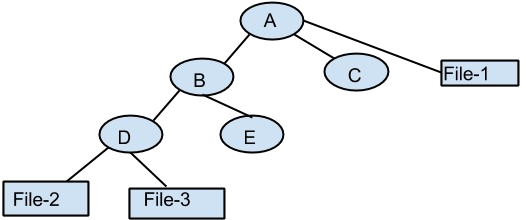
\includegraphics[scale=0.5]{figs/preliminar/FileSystemExample.png}
  \caption{Sample File System Tree}
  \label{fig:ExampleFileSystem}
\end{figure}


\begin{table}[!h]
\textbf{ACTIONS}\\

\begin{tabular}{|c|p{4cm}|c|p{8cm}|}
\hline
Directory&Opeartion&Time&Comments\\
\hline
A&Take Snapshot on A&1& \\
\hline
E&Create file F4&2&Insert row in Inodes table for F4 with parent E\\
\hline
E&Create file F5&3&Insert row in Inodes table for F5 with parent E.\\
\hline
D&Delete File F2&4&
1)Insert row in d-list. 2)set isDeleted=1 on Inodes table.\\
\hline
A&Take Snapshot on A&5& \\
\hline
D&Create File F6&6&Insert row in Inodes table for F6 with parent D\\
\hline
D&Move File F1 to C&7&1)Insert row in MV-LIST.
 2)Insert row in MV-IN-LIST Table.
 3)Change the parent\_ id to 3 for F4 in inodes table.\\
\hline
\end{tabular}
\caption{Operations}
\label{table:Actions}
\end{table}
\pagebreak

\begin{table}[!h]
\textbf{SNAPS}\\

\begin{tabular}{|c|c|c|c|}
\hline
Inode\_ Id&User&Snapshot\_ id&Time\\
\hline
A&Admin&SA1&1\\
\hline
A&Admin&SA2&5\\
\hline
\end{tabular}
\caption{List of Snpashots taken}
\label{table:snaps}
\end{table}


\begin{table}[!h]
\textbf{C-List}\\

\begin{tabular}{|c|c|c|}
\hline
Inode\_ Id&Time&Created\_ Node\_ Id\\
\hline
E&2&F4\\
\hline
E&3&F5\\
\hline
D&6&F6\\
\hline
\end{tabular}
\caption{C-List}
\label{table:clist}
\end{table}

\begin{table}[!h]
\textbf{D-List}\\

\begin{tabular}{|c|c|c|}
\hline
Inode\_ Id&Time&Deleted\_ Node\_ Id\\
\hline
D&4&F2\\
\hline
\end{tabular}
\label{table:dlist}
\caption{Dlist}
\end{table}

\begin{table}[!h]
\textbf{MV-List}\\

\begin{tabular}{|c|c|c|c|}
\hline
Inode\_ Id&Time&Moved\_ Node\_ Id&Original Row\\
\hline
A&7&F1&Orignal Row before moving\\
\hline
\end{tabular}
\caption{MV List}
\label{table:mvlist}
\end{table}


\textbf{MV-IN-List}\\

\begin{tabular}{|c|c|c|}
\hline
Inode\_ Id&Time&MovedIn\_ Node\_ Id\\
\hline
C&7&F1\\
\hline
\end{tabular}


\pagebreak

\subsection{Listing children under a directory in a given Snapshot}
To get the subtree under a directory at a particular snapshot, we use the following pseduo algorithm called with directory id and the time at which snapshot was taken. The algorithm presented here gives a general idea, the implementation in sql\cite{Snapshot-ls} addresses/solves the fine grained issues, for example, inode created after snapshot, moved, then moved-in, like those cases.

\begin{verbatim}
void ls_at_snapshot(int id, int stime){

    children={Get children whose parentId=id};
    children = childen - { children deleted before stime} -{ children created after stime} 
                        - {children moved_in 	after stime};
    children = children + {children moved-out after stime};
    modifiedChildren = { children modified after stime};

    for(child chd : children){
    	    child inode;
        if(modifiedChildren.contains(chd)){
            modChd = modifiedChildren.get(chd.getId());
            if(chd.movedTime>modChd.modifiedTime){
                #This child modified first then moved.So return the row stored M-List with modChd.modifiedTime
                inode = modChd;             
            }
            else{
               inode = chd;.
            }
    	   }
    	   else{
    	         inode = chd;
    	   }
    	   
    	   if(inode is directory){
    	        ls+at_snapshot(inode.getId(),stime);
    	   }
    	   else{
    	       print(inode);
    	   }
    }
}

\end{verbatim}

\subsection{Listing current children under a directory }
For listing current subtree under a directory, we select children which are not deleted.\\
\begin{verbatim}
void ls_current(int id){
    children={Get children whose parentId=id};
    children = childen - { children isDeleted=1}; 

    for(child chd : children){
    	    if(inode is directory){
    	        ls_current(inode.getId());
    	   }
    	   else{
    	       print(inode);
    	   }
    }
}
\end{verbatim}

\subsection{Logging, Removing logs and Deleting inodes which are not referred by any snapshot}
\label{loggingApproaches}
Here two approaches two solve the issues are presented.
\subsubsection{Approach 1:}
\textbf{Columns to be added to Inodes Table}\\
1. Moved\_ In/Created Time(Join Time): When an Inode is created we put that time in that column. When we move an Inode from one directory to another we note that time in that.We refer it as join time meaning the time this inode joined in its present directory.\\\\
\textbf{InodeSnapshotMap}\\
\begin{table}[h!]
\begin{tabular}{|c|c|c|c|}
\hline
Inode\_ Id&
BelongedTo\_ inode\_ id&
BeginTime&
EndTime\\
\hline
\end{tabular}\\
\caption{InodeSnapshotMap table}
\label{movedPaths}
\end{table}


\textbf{When to Log}\\
 When we add/ deleted/modify directories or files in a directory then we log changes under that directory. We log only when this directory is in any snapshot[which is taken on this directory or one-of its ancestors]. So before performing any operation in this directory we check whether this directory is in any snapshot or not.Consider directory path /A/B/C/, we want to add a file to directory C.We can log this in C-List if C is in a snapshot. \\
 1. First Check any snapshots taken on C.If yes then log.\\
 2. Get the Join-Time of each inode on the path i.e A,B,C and select the maximum time. If there are any snapshots taken on A or B after maximum time then log.\\
 3. If there is any entry for C in InodeSnapshotMap then log.\\
\\
\textbf{Moving an Inode}\\ 
Consider directory paths /A/B/ and /U/V/W/, move directory W to B.
\begin{enumerate}
\item Get the list of snapshots taken on U,V after the join time of W. In the form like
\{U,Time of First Snapshot after Join Time, Time Last Snapshot after Join Time\}.
\item Since some inodes under W may have join times greater than W' join time, we need to check for each inode in sub-tree on which snapshots of U,V is present.After determining which snapshots it is in then insert row in InodeSnapshotMap table.In this way we capture in which snapshots a particular inode is in when it is being moved. Here if we observe, the join times of inodes on directory path from root to child are non-decreasing.This enforces an order which is useful in finding whether an inode is in any snapshots or not.
\item Set the Join time of each children in the subtree to the present time.
\end{enumerate}

\textbf{Logging modifications of files and blocks:}\\
When we change any columns corresponding to the file in Inode table those were handled as mentioned above. If we append new blocks to or modify existing blocks then we should check whether to log them or not. This depends on whether this file is in any snapshot or not. So we follow the similar procedure as mentioned above.

%\textbf{Deleting logs}\\
 %We follow the same approach as mentioned in the %Approach2.

\textbf{Deletion of a file/or directory}\\
When the issuer issues command to delete a file, first , we check whether it is in any snapshot, if not then we permanently delete it.When deleting a directory, if it is in snapshot,we mark all the children with isDeleted=1 and the background delete thread will do check on inodes , deleting those not present in any snapshot permanently.Consider /A/B/C/ suppose want to delete C. First get the list of snapshots on A,B after the join time of C then for each child in sub-tree rooted at C set isDeleted=1, also inserting rows in inodesMap table based on the join time of child with the list of snapshots on A,B after join time of C. When you are deleting an inode permanently delete the logs associated with it in tables c-list,d-list,etc..

\textbf{Deleting entries in MovedPaths Table}\\
When we delete a snapshot on an inode, we check for entries in InodeSnapshotMap with that can be deleted.

\subsubsection{Approach :2}
When snapshot is taken we place the inodes under the snapshot in below table.

\begin{tabular}{|c|c|}
\hline
Inode\_ Id&Snapshot\_ time\\
\hline
\end{tabular}\\\\
if an inode with isDeleted=true and there is no entry in the above table , then we can remove that file from HDFS permanently.\\
The tables M-List, D-List, C-list , MV-list and MV-IN-List are populated for a directory when it is in a snapshot means an entry can be found in the above table.\\\\
\textbf{Cleaning the logs when a Snapshot is Deleted}\\
When a snapshot is deleted, all inodes under that snapshot can delete their logs on a criteria explained shortly. 1,2..numbers represent files in a directory P. S1,S2,S3 represent snapshots taken in increasing chronological manner. As per the query to list files at a certain snapshot, say S2 , we get all inodes from inodes table whose parent is P then remove all the files created after taking snapshot and adjust those which are moved out , modified. Then remove files deleted before taking snapshot 

to get files at S2 for directory P ==$>$ \{1,2,3,4,5,6,7,8\} - \{3,4\}-\{7,8\} =\{1,2,5,6\}
It means, a snapshot at time T1requires logs in C-List, M-List, MV-List, Mv-In-List after time T1 and logs in D-List before T1.

When we delete a snapshot S , then for each inode under it we execute following algorithm.\\\\
\textbf{ALGORITHM}\\
if(S is first snapshot in which this inode is present when all snapshots in which it is present are arranged in chronological manner) then;\\
\hspace{5em}delete D-List Logs before S. delete logs in C-List, M-List, MV-List, Mv-In-List until next snapshot.

For example: If we delete S1, then delete logs in D-List before S1, and logs in C-List, M-List, MV-List, MV-IN-List in between S1 and S2.\\

\begin{figure}[h!]
\centering  
 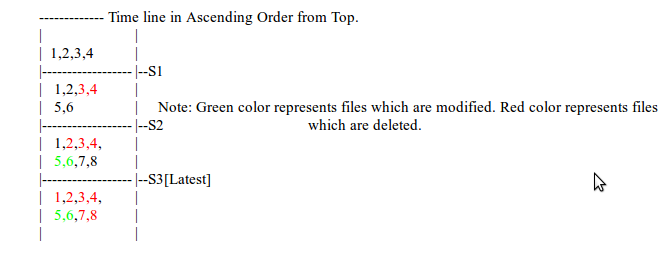
\includegraphics[scale=0.8]{figs/preliminar/Approach2.png}
  \caption{Deletion of Snapshot}
  \label{fig:approach2}
\end{figure}


\textbf{Deleting an file/Inode}\\
If the file is with isDeleted=1 and there is no entry for it in above table then it can be deleted permanently. After deleting file, we will check in D-List, to see if there are any logs with this Inode, if there then we will delete them.The same applies for directory. When user issues a command to delete a directory then mark isDeleted=1 for all of its children.Each children is an Inode, so we If the Inode is with isDeleted=1 and there is no entry for it in above table then it can be deleted permanently. After deleting Inode, we will check in D-List, to see if there are any logs with this Inode, if there then we will delete them

\textbf{Handling the replication factor change of a file}\\
Since we keep latest information about an Inode in Inodes’ table, we need to a mechanism to handle the case of replication factor changes. For example, in S1 the replication factor is 3 , then changed to 6 and S2 was taken , then changed to 9 , then S3 was taken, then changed to 2.
We find value 2 in Inodes’ table. The replication factor= Max(Current value, Max(values in M-List for this Inode)). In this case we will find it as 9 and we expect block report mentioning replication factor of 9 for each block.Suppose S3 was deleted , then the row with value 9 is deleted and we find maximum value 6. 

\textbf{Disadvantages:}\\
1. Time for taking snapshot is O(n) where n is the number of descendants  in directory \\
2. The space overhead on taking snapshot is o(n) where n is the number of descendants in directory.

\subsection{Length of file being Written}
This section explains the case when snapshot was taken while writing to file is in progress.In HDFS file System metadata and actual data are separated and store at different places.Various options to know the length of the file are:
\begin{enumerate}
 \item Length of all completed/finalized blocks and zero length considered from block under
construction.
\item Length when block is closed after snapshot creation occurred.
\item Length as seen at or around the time of snapshot creation in NameNode.
\begin{itemize}
 \item Either, DataNode reports the length in heartbeat or other commands
\item  Or, NameNode queries the length
\end{itemize}

\item Namenode and Datanodes could have communication to establish the snapshot length after
snapshot command is received by the namenode. But this is very complicated to implement
because of the distributed nature and the failure modes.
\item Client that care about the length of a file being written, could update length to the namenode as part of hflush/hsync. This is the length that gets recorded in the snapshot.
\item “Precise length” of the file at the time of snapshot creation.

\end{enumerate}

Clearly (6) is not possible given namespace and data block storage separation. Any guarantees in this regard will not be useful for the application, given that an application will need this consistency across many files that are part of the snapshot. \\
(1) Does not capture any changes that has occurred in the file from the time of new
block creation to the time of snapshot command. This is a good choice only if an application is willing to close the files before creating snapshots. That means application must have control over the data being written to the files and also snapshot creation. This may not be useful for HBase.\\
(2) will not be acceptable for many applications. Some reasons being - a file could be slowly written to and may not close for a long time. What is the length of such files in snapshot? Secondly, length of the file changes post snapshot - what guarantee is HDFS providing in terms of snapshot creation time?\\
(5)has the advantage that only applications that care about the correct length to be recorded in a snapshot use the hflush/hsync operation to report the length to the NN.

In both Read only Root Level Snapshot and Read only Nested Snapshots, (5) is chosen to implement.\\

\section{Read-Only Root Level Single Snapshot}
%\addcontentsline{lof}{chapter}{\thechapter\quad Lorem Ipsum}
%\addcontentsline{lot}{chapter}{\thechapter\quad Lorem Ipsum}


Following conditions are applied to the solution
\begin{enumerate}
\item Creation of directories with Quota, either name-space quota or disk-space quota is not allowed.
\item Each file consists of blocks. Each blocks-size is typically 64 MB but can be set to any value.Blocks should be written completely.
\end{enumerate}


  %%%%%%%%%%%%%%%%%%%%%%%%%%%%%%%%%%%%%%%%%%%%%%%%%%%%%%%%%%%%%%%%%%%%%%%%%%%%%
  %
%%%%%                        FIRST SECTION
 %%%
  %

\subsection{Modifications to the Schema}

Following columns need to be added to the Inodes table described in the schema \ref{fig:HDFS_table_schema} of HOP File System.
\begin{enumerate}
\item isDeleted \\\\
\begin{tabular}{|c|p{15cm}|}
\hline
Value&Summary\\
\hline
0&Indicates that this Inode is not deleted.\\
\hline
1&Indicates that this Inode deleted after Root Level snapshot was taken.\\ 
\hline
\end{tabular} \\
\item status \\\\
\begin{tabular}{|c|p{15cm}|}
\hline
Value&Summary\\
\hline
0&Indicates that this Inode was created before taking Root Level Snapshot.\\
\hline
2&Indicates that this Inode created before taking Root Level snapshot but modified after that.\\ 
\hline
3&Indicates that this Inode was created after taking Root Level snapshot.\\ 
\hline
\end{tabular} \\

\end{enumerate}
\pagebreak

Following Columns should be added to BlockInfos table described in the schema \ref{fig:HDFS_table_schema}.
\begin{enumerate}
\item status \\\\
\begin{tabular}{|c|p{15cm}|}
\hline
Value&Summary\\
\hline
0&Indicates that this Block was created before taking Root Level Snapshot.\\
\hline
2&Indicates that this Block created before taking Root Level snapshot but modified after that.\\ 
\hline
3&Indicates that this Block was created after taking Root Level snapshot.\\ 
\hline
\end{tabular} \\
\end{enumerate}

\subsection{Rules for Modifying the fileSystem meta-data}
Following rules apply when client issues operations described on \ref{NameNode_Ops} after root level snapshot had been taken.\\
HOP-HDFS as well as Apache HDFS allow only appends at the end of file.Both allow overwriting of an existing file.
\begin{enumerate}
\item If an inode(file or directory) is created after taking root level snapshot, its status is set to 3.
\item If an inode row is modified and its status is 0, then, a back-up of current row is saved with id = -(current id), parent\_ id=-(current parent\_ id)[To prevent sql query retrieving the back-up rows while 'ls' command issued, parent id is set to negative of original].The status of current row is changed to 2.
\item If a block is created after taking root level snapshot,its status is set to 3.
\item If a block is modified by appending data to it and its status is 0, then, a back-up of current row is saved with block\_ id = -(current block\_ id) and inode\_ id = -(current inode\_ id)[since two block info rows can't have same block index id when retrieved with a parent id].The status of current row is changed to 2.
\item Deletion of a directory or file after root level snapshot was taken.
Children of the INode to be deleted are examined in depth-first manner.All the  files which are created after snapshot was taken are permanently deleted.The directory's isDeleted flag is set to true.
\pagebreak
%\begin{verbatim}
%void deleteWithSnapshotAtRootTaken(INode targetNode){
%
%        Stack<INode> stck = new Stack<INode>();
%        INode tempNode;
%        List<INode> children;
%        INode[] inodesTemp;
%        INode removedInode;
%
%        stck.add(targetNode);
%
%        while (!stck.empty()) {
%            tempNode = stck.pop();
%            tempSts = tempNode.getStatus();
%            tempStr = tempNode.getFullPathName();
%           
%            if (tempNode.getIsDeleted() == 1) {
%                //This node is already marked deleted, so nothing to do.
%                continue;
%            }
%            /*
%             * This Inode can be a directory or file also it can be new or modified or original.
%             */
%            if (tempNode instanceof INodeDirectory) {
%                children = ((INodeDirectory) tempNode).getChildren();
%                if (children != null && !children.isEmpty()) {
%                    stck.push(tempNode);
%                    for (INode n : children) {
%                        stck.push(n);
%                    }
%                } else {
%                    if(tempNode.getStatus()==SnapShotConstants.New){
%                        //delete completely this directory Inode
%                        EntityManager.remove(tempNode);
%                    }
%                    else{
%                    //Set isDeleted = 1.
%                        tempNode.setIsDeletedNoPersistance(SnapShotConstants.isDeleted);
%                    }
%                }
%            } else if (tempNode instanceof INodeFile || tempNode instanceof INodeSymlink) {
%                if (tempSts == SnapShotConstants.New) {
%                    //We can delete this file permanently and update the ansectors about changes in the quota.
%                    //Remove the blocks associated with this file permanently.
%                    }
%                } else if (tempSts == SnapShotConstants.Original || tempSts == SnapShotConstants.Modified) {
%                    //Set isDeleted = 1.
%                    tempNode.setIsDeletedNoPersistance(1);
%                }
%            } 
%        }// End of while loop
%     }//End of method      
%            
%\end{verbatim}


\begin{verbatim}
void deleteWithSnapshotAtRootTaken(INode targetNode){

        Stack<INode> stck = new Stack<INode>();
        //parentStck is used to track completion of processing of a directory.
        Stack<INode> parentStck = new Stack<INode>();
        INode tempNode;
        List<INode> children;
        INode[] inodesTemp;
        INode removedInode;

        stck.add(targetNode);
        atomic{
           targetNode.setIsDeleted=1;   
        } 
        while (!stck.empty()) {
            tempNode = stck.pop();
            tempSts = tempNode.getStatus();
            tempStr = tempNode.getFullPathName();
           
            
            /*
             * This Inode can be a directory or file also it can be new or 
             modified or original.
             */
            if (tempNode instanceof INodeDirectory) {
                if(parentStack.top().equals(tempNode)){
                    //Processing children is completed
                    parentStack.pop();
                    if(tempNode.getStatus()==SnapShotConstants.New){
                         //delete completely this directory Inode
                        EntityManager.remove(tempNode);
                    }                
                
                }
                
                else{
                    parentStack.push(tempNode);            
                    children = ((INodeDirectory) tempNode).getChildren();
                    if (children != null && !children.isEmpty()) {
                        stck.push(tempNode);
                        for (INode n : children) {
                            stck.push(n);
                        }
                    } 
               }
           } else if (tempNode instanceof INodeFile ||
                         tempNode instanceof INodeSymlink) {
                         
                 if (tempSts == SnapShotConstants.New) {
                    atomic(In Single-Transaction){
                     //We can delete this file permanently and 
                     //update the ancestors about changes in the quota.
                     //Remove the blocks associated with this file
                     // permanently.
                     }
                 }
             } 
             
        }// End of while loop
        
		      
        
     }//End of method      
            
\end{verbatim}


\item Renaming/Moving an INode(File or Directory)
\begin{verbatim}
void renameINode(INode src, INode dst){
        1. Update the modification time of parent of src.
        2. Update the modification time of parent of dst.
        3. deletWithSnapshotAtRootTaken(dst).
        4. Change the parent\_ id of src to dst.parent\_ id.
}
\end{verbatim}

\end{enumerate}


  %%%%%%%%%%%%%%%%%%%%%%%%%%%%%%%%%%%%%%%%%%%%%%%%%%%%%%%%%%%%%%%%%%%%%%%%%%%%%
  %
%%%%%                      SECOND SECTION
 %%%
  %

\subsection{Roll Back}
 Following algorithm is used to roll back the file-system to the state at the time when Root Level Snapshot was taken.\\\\
For INodes:
\begin{enumerate}
\item Delete from INodes where status=2 or status=3
\item Update INodes set isDeleted=0 where id$>$0 and isDeleted=1
\item Update INodes set id = -id, parent\_ id = -parent\_ id where id$<$0
\end{enumerate}
For Blocks:
\begin{enumerate}
\item Delete from Block\_ Info where status=2 or status=3
\item Update Block\_ Info set block\_ id = -block\_ id, inode\_ id = -inode\_ id where id$<$0
\item Delete from Block\_ Info where block\_ id$<$0
\end{enumerate}
\label{alg:ROSSRB}

\section{Implementation Details}

\subsection{RollBack Algorithm Implementation}
\label{RollBackImpl}
With ClusterJ it is implemented as below.\\
1. Take the write lock on root so that no subtree operations under root can be allowed after rollBack command issued.
  \\ 1.1  Take read lock on all the inodes of the fileSystem, to make sure that there are no operations going on them while roll-back command issued.
\begin{verbatim}
DeleteRunnable(int start, int end) {
    void run(){
        //delete from inodes where status=2 or status=3 and id>=start 
        and id<=end;
        }
}

UpdateRunnableForCoulmnIsDeletd(int start, int end){
    void run(){

        //update inodes set isDeleted=0 where id>=start and 
        id<=end  and isDeleted=1;
        }
}

UpdateRunnableForColumnId(int start, int end,Lock lock){
void run(){
    List<INode> oldRows =  select * from inodes where id<=end and id>=start;
    List<INode> newRows = new ArrayList<INode>(oldRows.size());
        for(INode row: oldRows){
            INode updatedRow = session.instanceOf(INode.dto);
            updateRow.setId(-row.getId());
            updateRow.setParentId(-row.getParentId());
            //similarly other columns.
        }        
         Synchronized(lock){
            session.savePersistentAll(newRows);         
        }
       //delete from inodes where id>=start and id<=end;    
    }//end of run method
}

ThreadPool pool = new ThreadPool();
BatchSize=100,000;

Task1:
int maxId = select max(id) from inodes where status=2 or status=3;
int minId = select min(id) from inodes where status =2 or status=3;
int count=minId;

while(count<=maxId){
    pool.add(new DeleteRunnable(count,count+BlockSize);
    count = count+BlockSize;
}
//wait for completion of task.

Task2:

maxId = select max(id) from inodes where isDeleted=1 and id>0;
minId = select min(id) from inodes where  isDeleted=1 and id>0;
count=minId;

while(count<=maxId){
    pool.add(new UpdateRunnableForCoulmnIsDeletd(count,count+BlockSize);
    count = count+BlockSize;
}

//wait for completion of task.
Task3:

maxId = select max(id) from inodes where id<0;
minId = select min(id) from inodes where id<0;
count=minId;
Lock lock = new Lock();

while(count<=maxId){
    pool.add(new UpdateRunnableForColumnId(count,count+BlockSize,lock);
    count = count+BlockSize;
}

//wait for completion of task.

\end{verbatim}

\textbf{Failure Handling.}
For Task1, Task2 and Task3 , when a NameNode starts executing it will insert a row in Transaction with Task Id , NameNode Id,status. If status is InProgress and NameNode is dead, then the leader will direct other namnode to execute that task. There is a progress after each failure followed taking over by another namenode.

  %%%%%%%%%%%%%%%%%%%%%%%%%%%%%%%%%%%%%%%%%%%%%%%%%%%%%%%%%%%%%%%%%%%%%%%%%%%%%
  %
%%%%%                      SECOND SECTION
 %%%
  %



  %%%%%%%%%%%%%%%%%%%%%%%%%%%%%%%%%%%%%%%%%%%%%%%%%%%%%%%%%%%%%%%%%%%%%%%%%%%%%
  %
%%%%%                         ANOTHER SECTION
 %%%
  %


  %%%%%%%%%%%%%%%%%%%%%%%%%%%%%%%%%%%%%%%%%%%%%%%%%%%%%%%%%%%%%%%%%%%%%%%%%%%%%
  %
%%%%%                          LAST SECTION
 %%%
  %


  %
 %%%
%%%%%                        THE END
  %
  %%%%%%%%%%%%%%%%%%%%%%%%%%%%%%%%%%%%%%%%%%%%%%%%%%%%%%%%%%%%%%%%%%%%%%%%%%%%%

%%% Local Variables: 
%%% mode: latex
%%% TeX-master: "tese"
%%% End: 
